\section{Технологический раздел}
\subsection{Средства реализации}
Для написания данной работы был выбран язык C\#~\cite{cpp-lang}.
Этот выбор обусловлен следующими причинами:
\begin{itemize}
	\item C\# --- объектно-ориентированный язык, что соответствует методологии, выбранной для разработки программы;
	\item C\# предоставляется обширный набор библиотек и шаблонов, что позволяет использовать готовые конструкции и значительно экономит время разработки.
\end{itemize}

В качестве среды разработки был использован Visual Studio 2022~\cite{qt-creator}.
Данный выбор обусловлен следующими факторами:
\begin{itemize}
	\item в Visual Studio есть возможность быстрого создания интерфейса с помощью WinForms;
	\item Visual Studio предоставляет шаблоны, которые облегчают процесс написания и отладки проекта.
\end{itemize}

\subsection{Сведения о модулях программы}
Программы состоит из следующих модулей:
\begin{itemize}
	\item Program.cs --- точка входа в программу;
	\item Form.cs --- интерфейс программы;
	\item Station.cs --- описывает станцию;
	\item Platform.cs --- описывает платформу;
	\item Track.cs --- описывает путь;
	\item Train.cs --- описывает поезд.
\end{itemize}

\subsection{Реализация программы}
Ниже, на листингах 1--4, приведены реализации классов, сделанны студентом Ву Хай Данг.
\begin{lstlisting}[caption={Класс Station}, label={lst:station}]
public class Station
{
	private string name;
	private List<Platform> platforms;
	private List<Train> trains;
	
	public string Name { get => name; set => name = value; }
	public List<Platform> Platforms { get => platforms; set => platforms = value; }
	public List<Train> Trains { get => trains; set => trains = value; }
	
	public Station(string name, List<Platform> platforms)
	{
		this.name = name;
		this.platforms = platforms;
		this.trains = new List<Train>();
	}
	public void AddTrain(Train train)
	{
		this.trains.Add(train);
	}
	
	public void Schedule()
	{
		foreach (var train in trains.OrderBy(t => t.DepartureTime))
		{
			TimeSpan minTime = new TimeSpan(23, 59, 59);
			Platform platformTmp = null;
			Track trackTmp = null;
			foreach (var platform in platforms)
			{
				foreach (var track in platform.Tracks)
				{
					if ((train.Direction.Split(' ')[0] == "Moscow" && track.Direction == "From Moscow") ||
					(train.Direction.Split(' ')[0] != "Moscow" && track.Direction == "To Moscow"))
					{
						if (track.CurrTrains.Count == 0 ||
						(train.DepartureTime.TotalMinutes - track.CurrTrains.Last().
						DepartureTime.TotalMinutes) >= 9)
						{
							track.CurrTrains.Add(train);
							train.PlatformAssigned = platform.Id;
							train.TrackAssigned = track.Id;
							train.WasPlaned = true;
							train.setSpeed();
							break;
						}
						else
						{
							if (track.CurrTrains.Last().DepartureTime <= minTime)
							{
								minTime = track.CurrTrains.Last().DepartureTime;
								platformTmp = platform;
								trackTmp = track;
							}
						}
					}
				}
				if (train.WasPlaned)
				break;
			}
			if (!train.WasPlaned)
			{
				train.DepartureTime = TimeSpan.FromMinutes(minTime.TotalMinutes + 10);
				trackTmp.CurrTrains.Add(train);
				train.PlatformAssigned = platformTmp.Id;
				train.TrackAssigned = trackTmp.Id;
				train.WasPlaned = true;
				train.setSpeed();
			}
			
		}
	}
	
	public void UpdatePlatforms(int width)
	{
		foreach (var platform in platforms)
		{
			foreach (var track in platform.Tracks)
			{
				track.CurrTrains.RemoveAll(t => t.hasArrived(width) == true);
			}
		}
	}
}
\end{lstlisting}

\begin{lstlisting}[caption={Класс Platform}, label={lst:platform}]
public class Platform
{
	private int id;
	private List<Track> tracks;
	public int Id { get => id; set => id = value; }
	internal List<Track> Tracks { get => tracks; set => tracks = value; }
	
	public Platform(int id, List<Track> tracks)
	{
		this.id = id;
		this.tracks = tracks;
	}
}
\end{lstlisting}

\begin{lstlisting}[caption={Класс Track}, label={lst:track}]
public class Track
{
	private int id;
	private string direction;
	private List<Train> currTrains;
	public int Id { get => id; set => id = value; }
	public List<Train> CurrTrains { get => currTrains; set => currTrains = value; }
	public string Direction { get => direction; set => direction = value; }
	
	public Track(int id, string direction)
	{
		this.id = id;
		this.direction = direction;
		this.CurrTrains = new List<Train>();
	}
}
\end{lstlisting}

\begin{lstlisting}[caption={Класс Train}, label={lst:train}]
public class Train
{
	private int id;
	private PictureBox pic = new PictureBox();
	private TimeSpan arrivalTime;
	private TimeSpan departureTime;
	private string direction;
	private string type;
	private int platformAssigned;
	private int trackAssigned;
	private bool hasDrawn = false;
	private bool wasPlaned = false;
	private int speed = 7;
	
	private int timeStoped = 50;
	static public int speedGlobal = 7;
	static public Dictionary<int, Point> positions = new Dictionary<int, Point>
	{
		{1, new Point(0, 71 + 177) },
		{2, new Point(1127, 115 + 177) },
		{3, new Point(0, 242 + 177) },
		{4, new Point(1127, 286 + 177) },
		{5, new Point(0, 428 + 177) },
		{6, new Point(1127, 472 + 177) }
	};
	
	public int Id { get => id; set => id = value; }
	public TimeSpan ArrivalTime { get => arrivalTime; set => arrivalTime = value; }
	public TimeSpan DepartureTime { get => departureTime; set => departureTime = value; }
	public string Direction { get => direction; set => direction = value; }
	public string Type { get => type; set => type = value; }
	public PictureBox Pic { get => pic; set => pic = value; }
	public int PlatformAssigned { get => platformAssigned; set => platformAssigned = value; }
	public int TrackAssigned { get => trackAssigned; set => trackAssigned = value; }
	public bool HasDrawn { get => hasDrawn; set => hasDrawn = value; }
	public int Speed { get => speed; set => speed = value; }
	public int TimeStoped { get => timeStoped; set => timeStoped = value; }
	public bool WasPlaned { get => wasPlaned; set => wasPlaned = value; }
	
	public Train(int id, TimeSpan departureTime, TimeSpan arrivalTime, string direction, string type)
	{
		this.id = id;
		pic.BackColor = Color.Red;
		pic.Location = new Point();
		pic.Size = new Size(100, 38);
		this.arrivalTime = arrivalTime;
		this.departureTime = departureTime;
		this.direction = direction;
		this.type = type;
	}
	
	public void MoveTrain()
	{
		var pos = pic.Location;
		pos.X += Speed;
		pic.Location = pos;
	}
	
	public void setSpeed()
	{
		if (trackAssigned % 2 == 0)
		Speed = -Speed;
	}
	public bool hasArrived(int width)
	{
		if (trackAssigned % 2 == 0)
		return pic.Location.X <= 0;
		else
		return pic.Location.X >= width;
	}
}
}
\end{lstlisting}

\subsection{Демонстрация работы программы}

На рисунках \ref{img:demon1}--\ref{img:demon2} приведен интерфейс программы,
сделанны студентом Фам Минь Хиеу.
\begin{figure}[h]
	\centering
	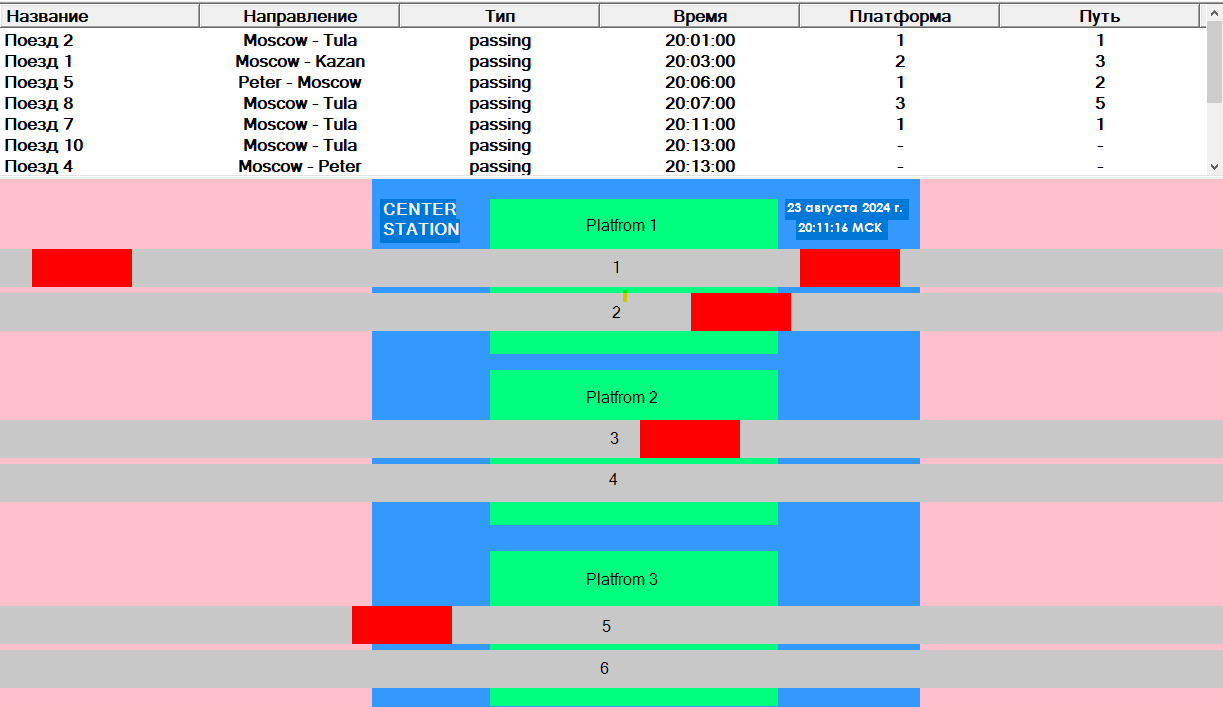
\includegraphics[height=0.35\textheight]{img/examples/demon1.png}
	\caption{Пример работы программы}
	\label{img:demon1}
\end{figure}

\begin{figure}[h]
	\centering
	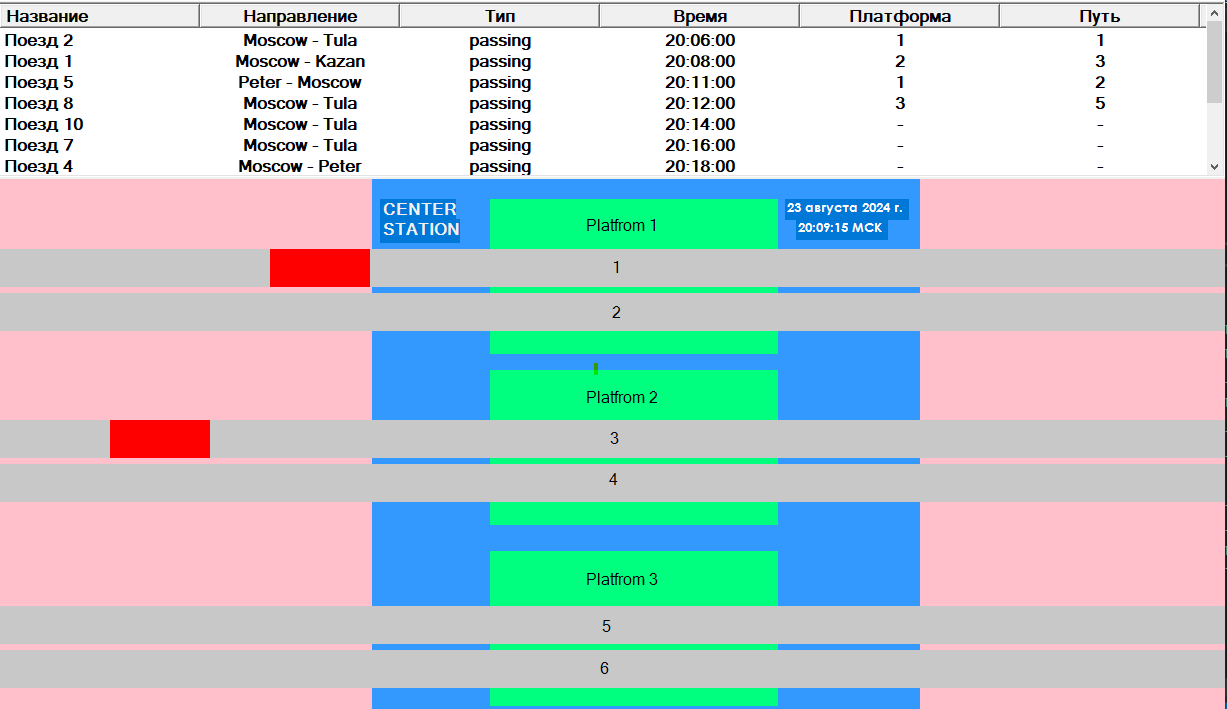
\includegraphics[height=0.35\textheight]{img/examples/demon2.png}
	\caption{Пример работы программы (продолжение)}
	\label{img:demon2}
\end{figure}
